\documentclass[11pt,a4paper]{article}
\usepackage{fontspec}
\setmainfont{DejaVu Serif}
\usepackage{amsmath,amssymb,graphicx,booktabs,geometry,hyperref}
\geometry{margin=22mm}
\sloppy
\setlength{\emergencystretch}{3em}
\begin{document}
\title{Експеримент 4: добір і незалежні форми}\author{}\date{2026-11-01}\maketitle

\section*{Протокол, зафіксований до оцінювання}
Навчальні форми: коло й квадрат; seeds $0,1,2$, Sobol по 512 точок,
$h=0.25$. Критерій --- RMSE у смузі $|d|<0.25$.
Кожен параметризований метод має не більше шести наперед заданих
кандидатів; linear/cubic/EDT мають один варіант без параметрів.
Грубий набір не гарантує оптимальності жодного методу.
Кандидат із відмовою хоча б на одній навчальній задачі не обирається.
Вибір збережено у \texttt{selection.json} перед фінальною перевіркою.

Незалежні форми: capsule, rounded box, перешийок, два диски,
сфера й тор. Capsule та rounded box додано як нові аналітичні SDF.
Seeds $10,11,12$ задають нові кути й зсуви.
Для 2D $h=0.2,0.3$, для 3D $h=0.4,0.5$; рівні $t=-0.1,0,0.1$.
Параметри з 2D переносяться в 3D без нового добору; це перевірка
перенесення, а не окремо оптимізовані 3D-методи.

\section*{Справедливість і вартість}
Спільні центри, float64, область $[-1,1]^D$, запас $4h$.
Кількість коефіцієнтів/значень однакова для основних методів.
Для $q=\|x-c\|/r$ використано
\[
 \phi_{C^2}(q)=(1-q)_+^4(4q+1),\qquad
 \phi_{C^4}(q)=(1-q)_+^6(35q^2+18q+3)/3.
\]
Це сімейства Вендланда для розмірностей 2/3; параметр $n$
у таблиці добору стосується лише псевдогаусового ядра.
Для Wendland наводяться окремо grid/isolines: додатна визначеність
при спільних вузлах не переноситься автоматично на зміщені вузли.
Cubic --- SciPy RegularGridInterpolator not-a-knot з прямим
розв'язувачем; linear --- білінійна/трилінійна інтерполяція.
Додатковий EDT-контроль: cubic витягується на сітку з кроком $h/2$,
потім знакова відстань EDT інтерполюється лінійно. Це окрема
дискретна baseline з додатковою пам'яттю та дрейфом поверхні.

Лічильники містять SDF API calls/points і projection calls/points;
аналітичні операції всередині проєктора не маскуються під однакову
вартість black-box запиту. Тому це однаковий максимум кандидатів,
а не гарантовано рівна кількість інформації про геометрію.
Час усіх кандидатів, включно з невдалими, включений у tuning time.
\begin{center}\small\resizebox{\linewidth}{!}{\begin{tabular}{llllllll}\toprule
Метод & $\rho$ & $n$ & $\Delta/h$ & Train RMSE & Добір, с & SDF points & Projection points\\\midrule
pg\_grid & 2 & 4 & 0.5 & 0.007414 & 0.07827 & 28836 & 0\\
pg\_isolines & 2 & 4 & 0.5 & 0.008186 & 0.126 & 49644 & 109242\\
wendland\_c2\_grid & 4 & -- & 0.5 & 0.006908 & 0.07799 & 28836 & 0\\
wendland\_c2\_isolines & 3 & -- & 0.5 & 0.009394 & 0.1092 & 49644 & 67626\\
wendland\_c4\_grid & 2.5 & -- & 0.5 & 0.007732 & 0.07808 & 28836 & 0\\
wendland\_c4\_isolines & 3 & -- & 0.5 & 0.009207 & 0.1084 & 49644 & 67626\\
linear & 2 & -- & 0.5 & 0.01495 & 0.001918 & 4806 & 0\\
cubic & 2 & -- & 0.5 & 0.006996 & 0.006578 & 4806 & 0\\
cubic\_redistance & 2 & -- & 0.5 & 0.06197 & 0.007918 & 4806 & 0\\
\bottomrule\end{tabular}}\end{center}

\section*{Результати на нових формах}
Таблиці --- медіани описових вимірювань, не незалежні статистичні
оцінки: кілька офсетів та h належать тій самій формі/seed.
Seed min/max --- діапазон медіан трьох окремих seeds, не довірчий
інтервал. За формами розкладено дані в by\_shape.json.
Відмови збережено, не замінено нульовою похибкою.
\begin{center}\small\resizebox{\linewidth}{!}{\begin{tabular}{lllllll}\toprule
2D метод & RMSE смуги & Seed min & Seed max & RMSE градієнта & $H_{sample}$ & Відмови\\\midrule
cubic & 0.01283 & 0.01256 & 0.01345 & 0.228 & 0.03872 & 0\\
cubic\_redistance & 0.0609 & 0.05913 & 0.06554 & 0.7248 & 0.1047 & 0\\
linear & 0.02288 & 0.02266 & 0.02319 & 0.3369 & 0.08571 & 0\\
pg\_grid & 0.01353 & 0.0131 & 0.01474 & 0.2301 & 0.03758 & 0\\
pg\_isolines & 0.01465 & 0.01454 & 0.01526 & 0.2422 & 0.04295 & 0\\
wendland\_c2\_grid & 0.01278 & 0.01276 & 0.01353 & 0.2275 & 0.03934 & 0\\
wendland\_c2\_isolines & 0.01377 & 0.01304 & 0.01427 & 0.2396 & 0.0415 & 0\\
wendland\_c4\_grid & 0.01325 & 0.01242 & 0.01331 & 0.2289 & 0.04177 & 0\\
wendland\_c4\_isolines & 0.01378 & 0.01341 & 0.0146 & 0.2399 & 0.04233 & 0\\
\bottomrule\end{tabular}}\end{center}
\begin{center}\small\resizebox{\linewidth}{!}{\begin{tabular}{lllllll}\toprule
3D метод & RMSE смуги & Seed min & Seed max & RMSE градієнта & $H_{sample}$ & Відмови\\\midrule
cubic & 0.01847 & 0.01794 & 0.01885 & 0.1848 & 0.04605 & 0\\
cubic\_redistance & 0.1058 & 0.1024 & 0.1081 & 0.9301 & 0.1482 & 0\\
linear & 0.06728 & 0.06697 & 0.06838 & 0.3461 & 0.1368 & 0\\
pg\_grid & 0.01946 & 0.01887 & 0.01983 & 0.2147 & 0.04658 & 0\\
pg\_isolines & 0.04961 & 0.04296 & 0.05427 & 0.4735 & 0.1635 & 0\\
wendland\_c2\_grid & 0.01769 & 0.01758 & 0.018 & 0.1711 & 0.04776 & 0\\
wendland\_c2\_isolines & 0.02273 & 0.02185 & 0.02396 & 0.1831 & 0.05361 & 0\\
wendland\_c4\_grid & 0.01553 & 0.01553 & 0.01608 & 0.1701 & 0.04102 & 0\\
wendland\_c4\_isolines & 0.02673 & 0.02578 & 0.02727 & 0.2017 & 0.06009 & 0\\
\bottomrule\end{tabular}}\end{center}
\begin{center}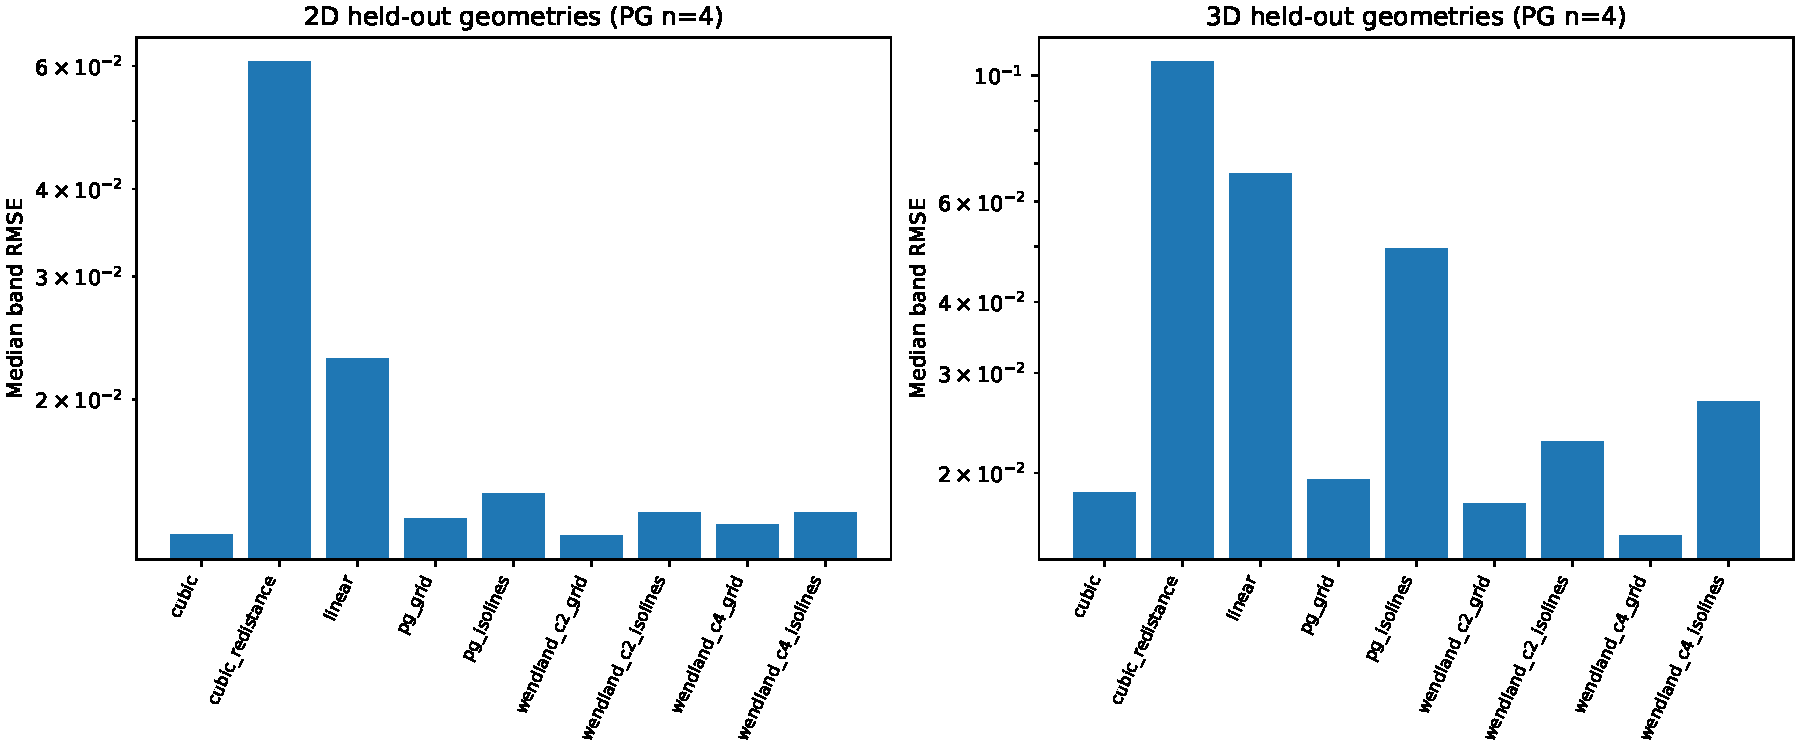
\includegraphics[width=\linewidth]{results/extended/holdout.pdf}\end{center}
\end{document}
